\documentclass[xcolor=pdftex,t,11pt]{beamer}


\usepackage{tipa}

\usetheme[
pagecounter=true,
pageofpages=of,  % page 7 "of" 9
bullet=circle,
titleline=true,
alternativetitlepage=true,
titlepagelogo=images/oxford_big_square,
% titlepagefooterlogo=images/oxford_small_square,
ordinarypageslogo=images/oxford_small_square,
% watermark=images/oxford_small_square,   % bottom right corner
% watermarkheight=100pt,
% watermarkheightmult=4,
]{Torino}
\usecolortheme{greenandblue}
\usefonttheme{structurebold}


\author{Volker Braun}
\title{Git and the New Sage Development Workflow}
\subtitle{Making distributed version control work for you}
\institute{Oxford University}
\date{September 23, 2013}

\begin{document}


\begin{frame}[plain]
	\titlepage
\end{frame}

\begin{frame}{Outline}
	\tableofcontents
\end{frame}



\section{Introduction}

\begin{frame}
  \frametitle{Git?!}
  

  \begin{block}{}
    git \textipa{/gIt/}\\
    \textit{v Appalachian \& southern US}\\
    \hspace{1cm} variant of \emph{get}\\
    \textit{n Brit slang pejorative}\\
    \hspace{1cm} foolish or worthless person
  \end{block}
  
\end{frame}



\begin{frame}[plain]
  \frametitle{Git Operations}
  \centering
  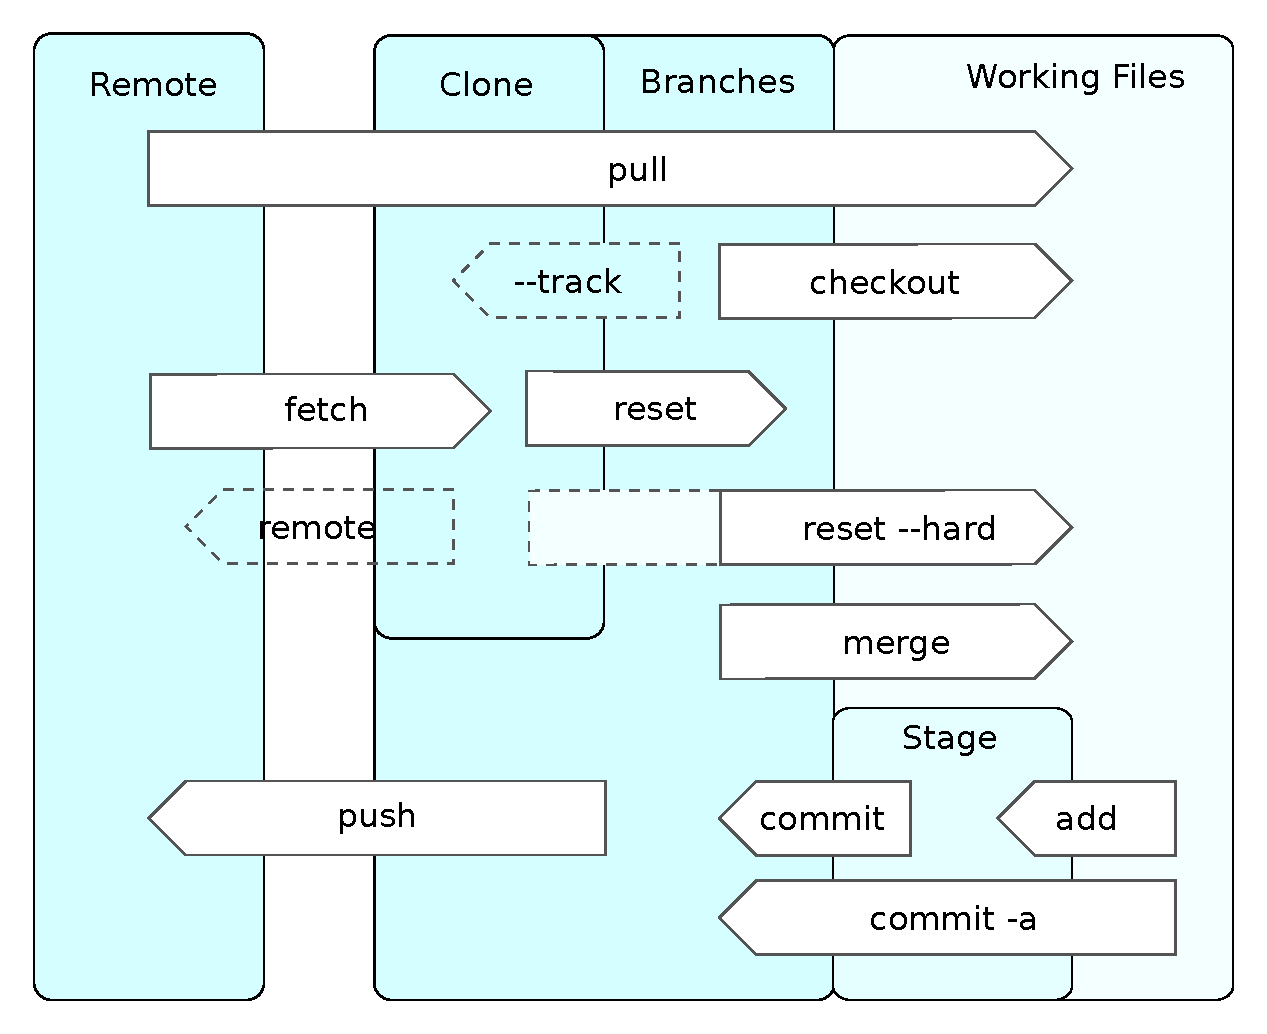
\includegraphics[width=0.85\linewidth]{images/git_operations}
\end{frame}


\end{document}